\documentclass{article}
\usepackage[letterpaper]{geometry}
\usepackage{tikz}
\usepackage{gensymb}
\usepackage{amssymb, amsmath, amsfonts}
\usetikzlibrary{intersections}

\begin{document}
	Unit Circle
	\\d
	\\
	\begin{center}
		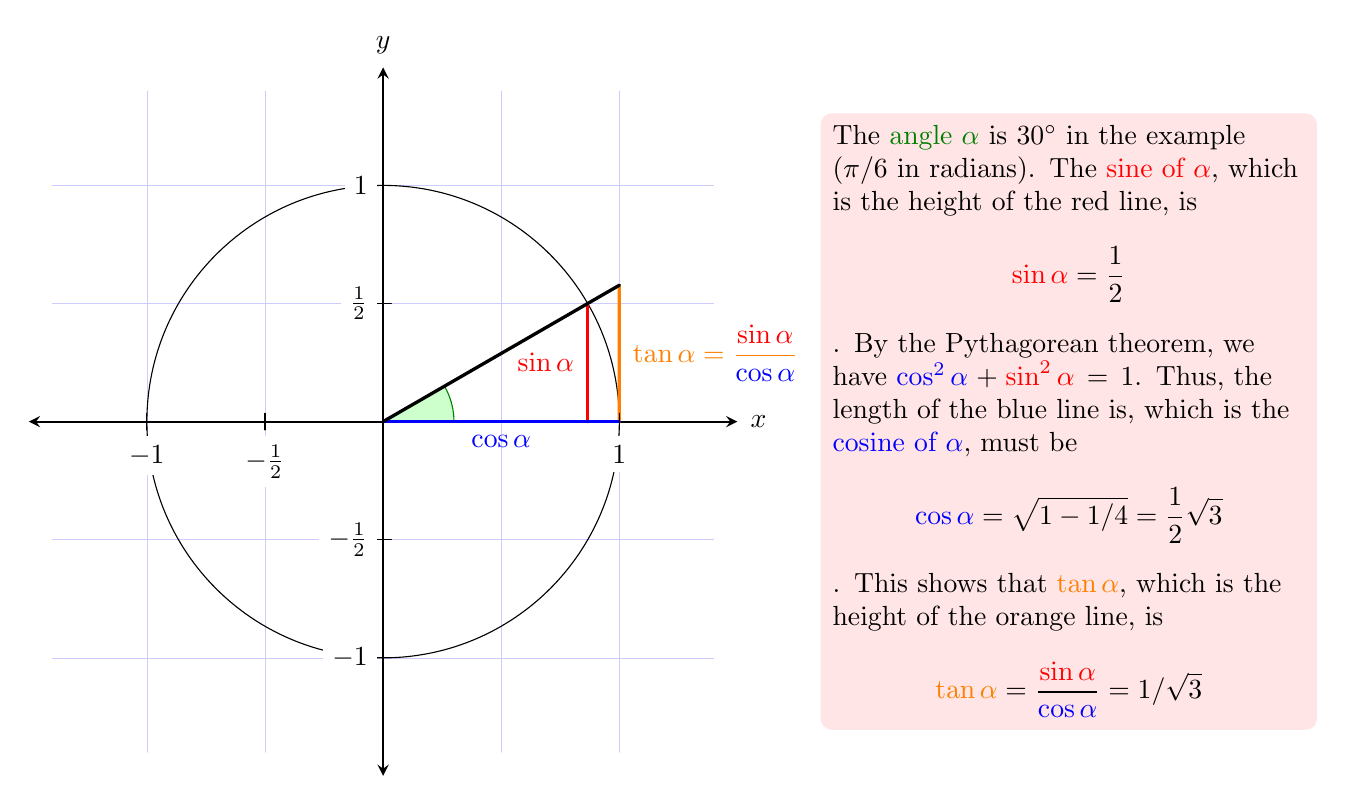
\begin{tikzpicture}
			[scale=3,
			>=stealth, 
			cap=round,
			information text/.style={rounded corners, fill=red!10, inner sep=1ex}]

			\draw[very thin, step=0.5cm, color=blue!20!white] (-1.4,-1.4) grid (1.4,1.4);
			
			\draw[thick,<->] (-1.5,0)--(1.5,0)node[right=1pt]{$x$};
			\draw[thick,<->]  (0,-1.5)--(0,1.5)node[above=1pt]{$ y $};
			
			\draw (0,0) circle (1cm);
			%\draw (3mm,0) arc (0:30:3mm);
			\filldraw[fill=green!20!white, draw=green!50!black] (0,0)--(3mm,0) arc (0:30:3mm)--cycle;
			
			\draw[very thick, red] (30:1cm)--node[left=1pt]{$\sin\alpha$}+(0,-0.5cm);
			
			\path[name path=upward line] (1,0)--(1,1);
			\path[name path=sloped line] (0,0)--(30:1.5cm);
			
			\draw[name intersections={of=upward line and sloped line, by=x}][very thick, orange] (1,0)--node[right=1pt]{$ \tan\alpha=\dfrac{\color{red}\sin\alpha}{\color{blue}\cos\alpha} $}(x);
			
			\draw[very thick, blue] (0,0)--node[below=1pt]{$\cos\alpha$}(1,0);
			
			\draw[very thick] (0,0)--(x);
			
			\foreach \y/\ytext in {-1, -0.5/-\frac{1}{2}, 0.5/\frac{1}{2}, 1}
				\draw[yshift=\y cm] (-1pt,0)--(1pt,0)node[left=5pt,	 fill=white]{$\ytext$};
				
			\foreach \x/\xtext in {-1,-0.5/-\frac{1}{2},1}
				\draw[xshift=\x cm] (0,1pt)--(0,-1pt)node[below=2pt, fill=white]{$ \xtext $};
			
			\draw[xshift=1.85cm]
				node[right, text width=6cm, information text]
				{The {\color{green!50!black}{angle $ \alpha $}} is $ 30\degree $ in the example ($ \pi/6 $ in radians). The {\color{red} sine of $ \alpha $}, which is the height of the red line, is {$${\color{red}\sin\alpha} =\dfrac{1}{2} $$}.
				By the Pythagorean theorem, we have $ {\color{blue}\cos^2{\alpha}}+{\color{red}\sin^2{\alpha}}=1 $. Thus, the length of the blue line is, which is the {\color{blue}cosine of $ \alpha $}, must be $$ {\color{blue}\cos\alpha}=\sqrt{1-1/4}=\frac{1}{2}\sqrt{3} $$. This shows that {\color{orange}$ \tan \alpha $}, which is the height of the orange line, is $${\color{orange}\tan\alpha} =\dfrac{\color{red}\sin\alpha}{\color{blue}\cos\alpha}=1/\sqrt{3} $$
				};

		\end{tikzpicture}
	\end{center}

	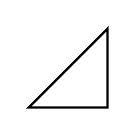
\begin{tikzpicture}
		\draw[thick] (0,0)--(1,0)--(1,1)--cycle;
	\end{tikzpicture}
	
\end{document}